\documentclass[aspectratio=169,11pt]{beamer}

% Theme configuration
\usetheme{Madrid}
\usecolortheme{default}
\setbeamertemplate{navigation symbols}{}
\setbeamertemplate{footline}[frame number]

% Required packages
\usepackage{graphicx}
\usepackage{booktabs}
\usepackage{amsmath}
\usepackage{amssymb}
\usepackage{hyperref}
\usepackage{tikz}
\usepackage{algorithm}
\usepackage{algpseudocode}

% Title information
\title{Natural Language Processing}
\subtitle{Course Overview and Introduction}
\author{Your Name}
\institute{Your Institution}
\date{\today}

\begin{document}

% Title slide
\begin{frame}
    \titlepage
\end{frame}

% Table of contents
\begin{frame}{Plan du cours}
    \tableofcontents
\end{frame}

% Introduction section
\section{Introduction au Traitement du Langage Naturel}

% First slide: Definition of NLP
\begin{frame}{Qu'est-ce que le NLP?}

    \begin{itemize}
        \item Le \textbf{Traitement du Langage Naturel (NLP)} est un domaine de l'intelligence artificielle qui se concentre sur l'interaction entre les ordinateurs et le langage humain
        \item Il vise à permettre aux machines de \textbf{comprendre}, \textbf{interpréter} et \textbf{générer} du langage humain
        \item Le langage est \textbf{omniprésent} dans notre monde:
        \begin{itemize}
            \item Livres, articles et documents
            \item Contenus web et réseaux sociaux
            \item Messages et conversations
            \item Emails et communications professionnelles
        \end{itemize}
        \item Le NLP nous permet d'exploiter et de donner du sens à cette ressource abondante
    \end{itemize}

\end{frame}

% Second slide: Applications of NLP - Text Understanding
\begin{frame}{Applications du NLP: Compréhension de texte}
    \begin{columns}
        \begin{column}{0.55\textwidth}
            \begin{itemize}
                \item \textbf{Analyse de sentiment}
                \begin{itemize}
                    \item Détection des opinions positives/négatives
                    \item Modération automatique des commentaires
                    \item Analyse des retours clients et avis
                \end{itemize}
                \vspace{0.3cm}
                \item \textbf{Classification de texte}
                \begin{itemize}
                    \item Catégorisation des emails (spam/non-spam)
                    \item Organisation des documents par thème
                    \item Filtrage de contenu inapproprié
                \end{itemize}
                \vspace{0.3cm}
                \item \textbf{Extraction d'information}
                \begin{itemize}
                    \item Reconnaissance d'entités nommées (noms, lieux, dates)
                    \item Extraction de relations entre entités
                    \item Résumé automatique de documents
                \end{itemize}
            \end{itemize}
        \end{column}
        \begin{column}{0.45\textwidth}
            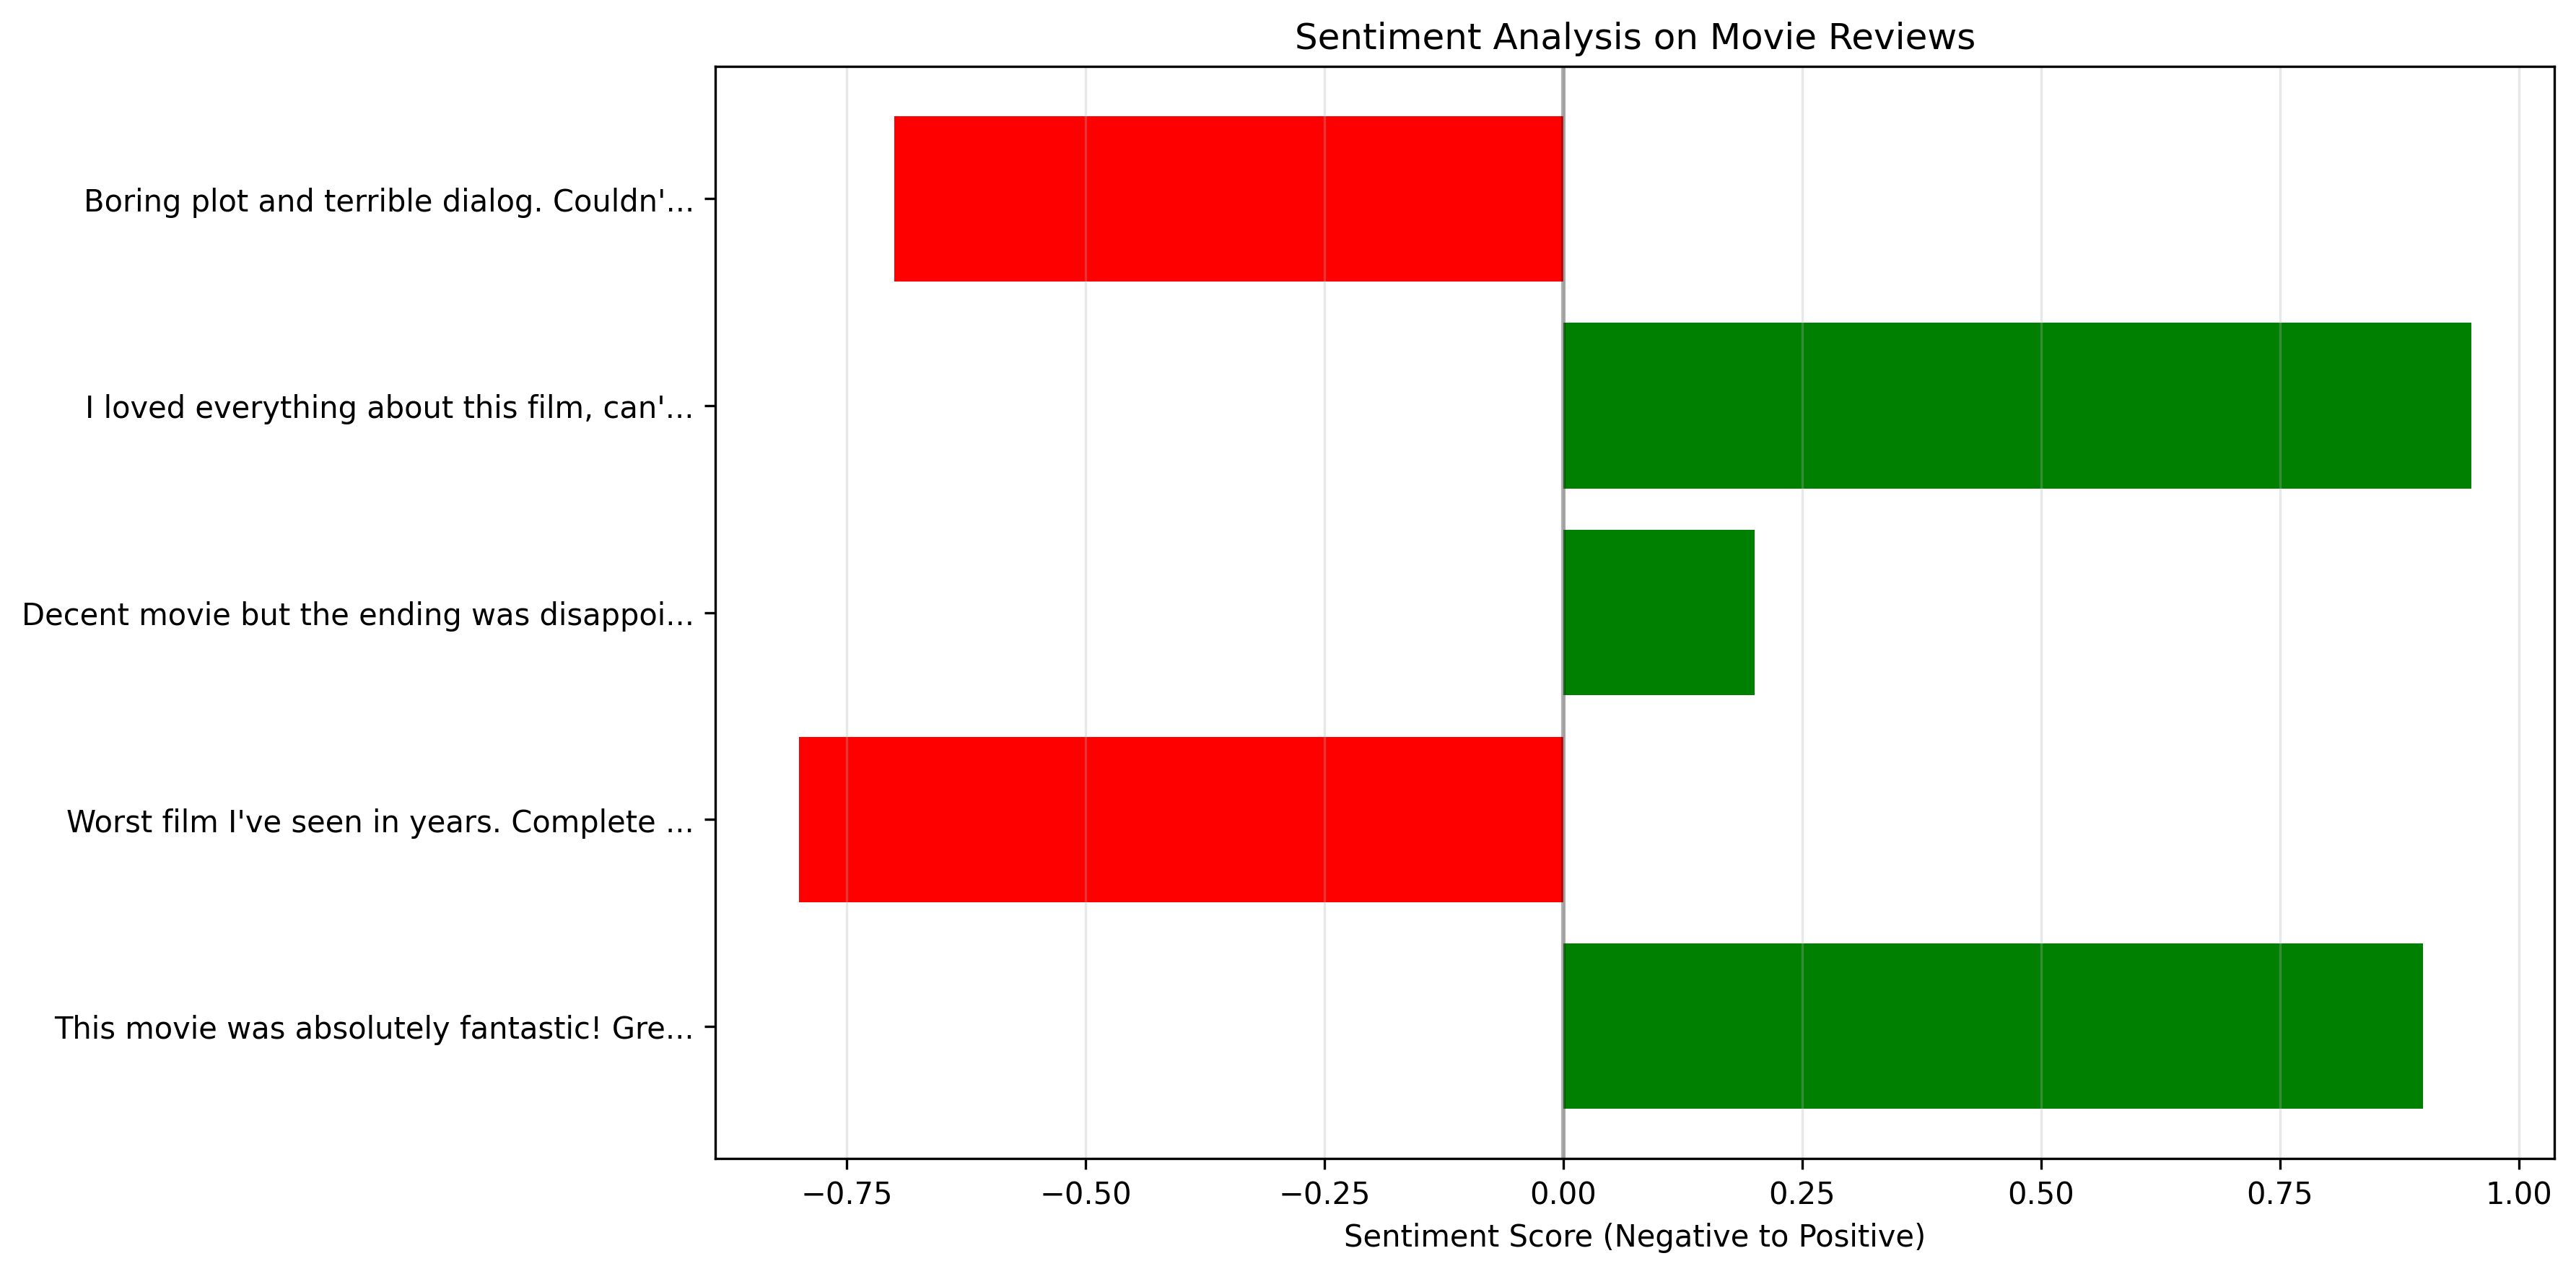
\includegraphics[width=\textwidth]{images/generated/sentiment_analysis.png}
            \vspace{0.5cm}
            \begin{center}
                \small{Exemple d'analyse de sentiment sur des critiques de films}
            \end{center}
        \end{column}
    \end{columns}
\end{frame}

% Third slide: Applications of NLP - Translation and Chatbots
\begin{frame}{Applications du NLP: Traduction et Assistants}
    \begin{columns}
        \begin{column}{0.5\textwidth}
            \textbf{Traduction automatique}
            \begin{itemize}
                \item Traduction instantanée entre langues
                \item Facilite la communication internationale
                \item Applications: Google Translate, DeepL
            \end{itemize}
            \vspace{0.3cm}
            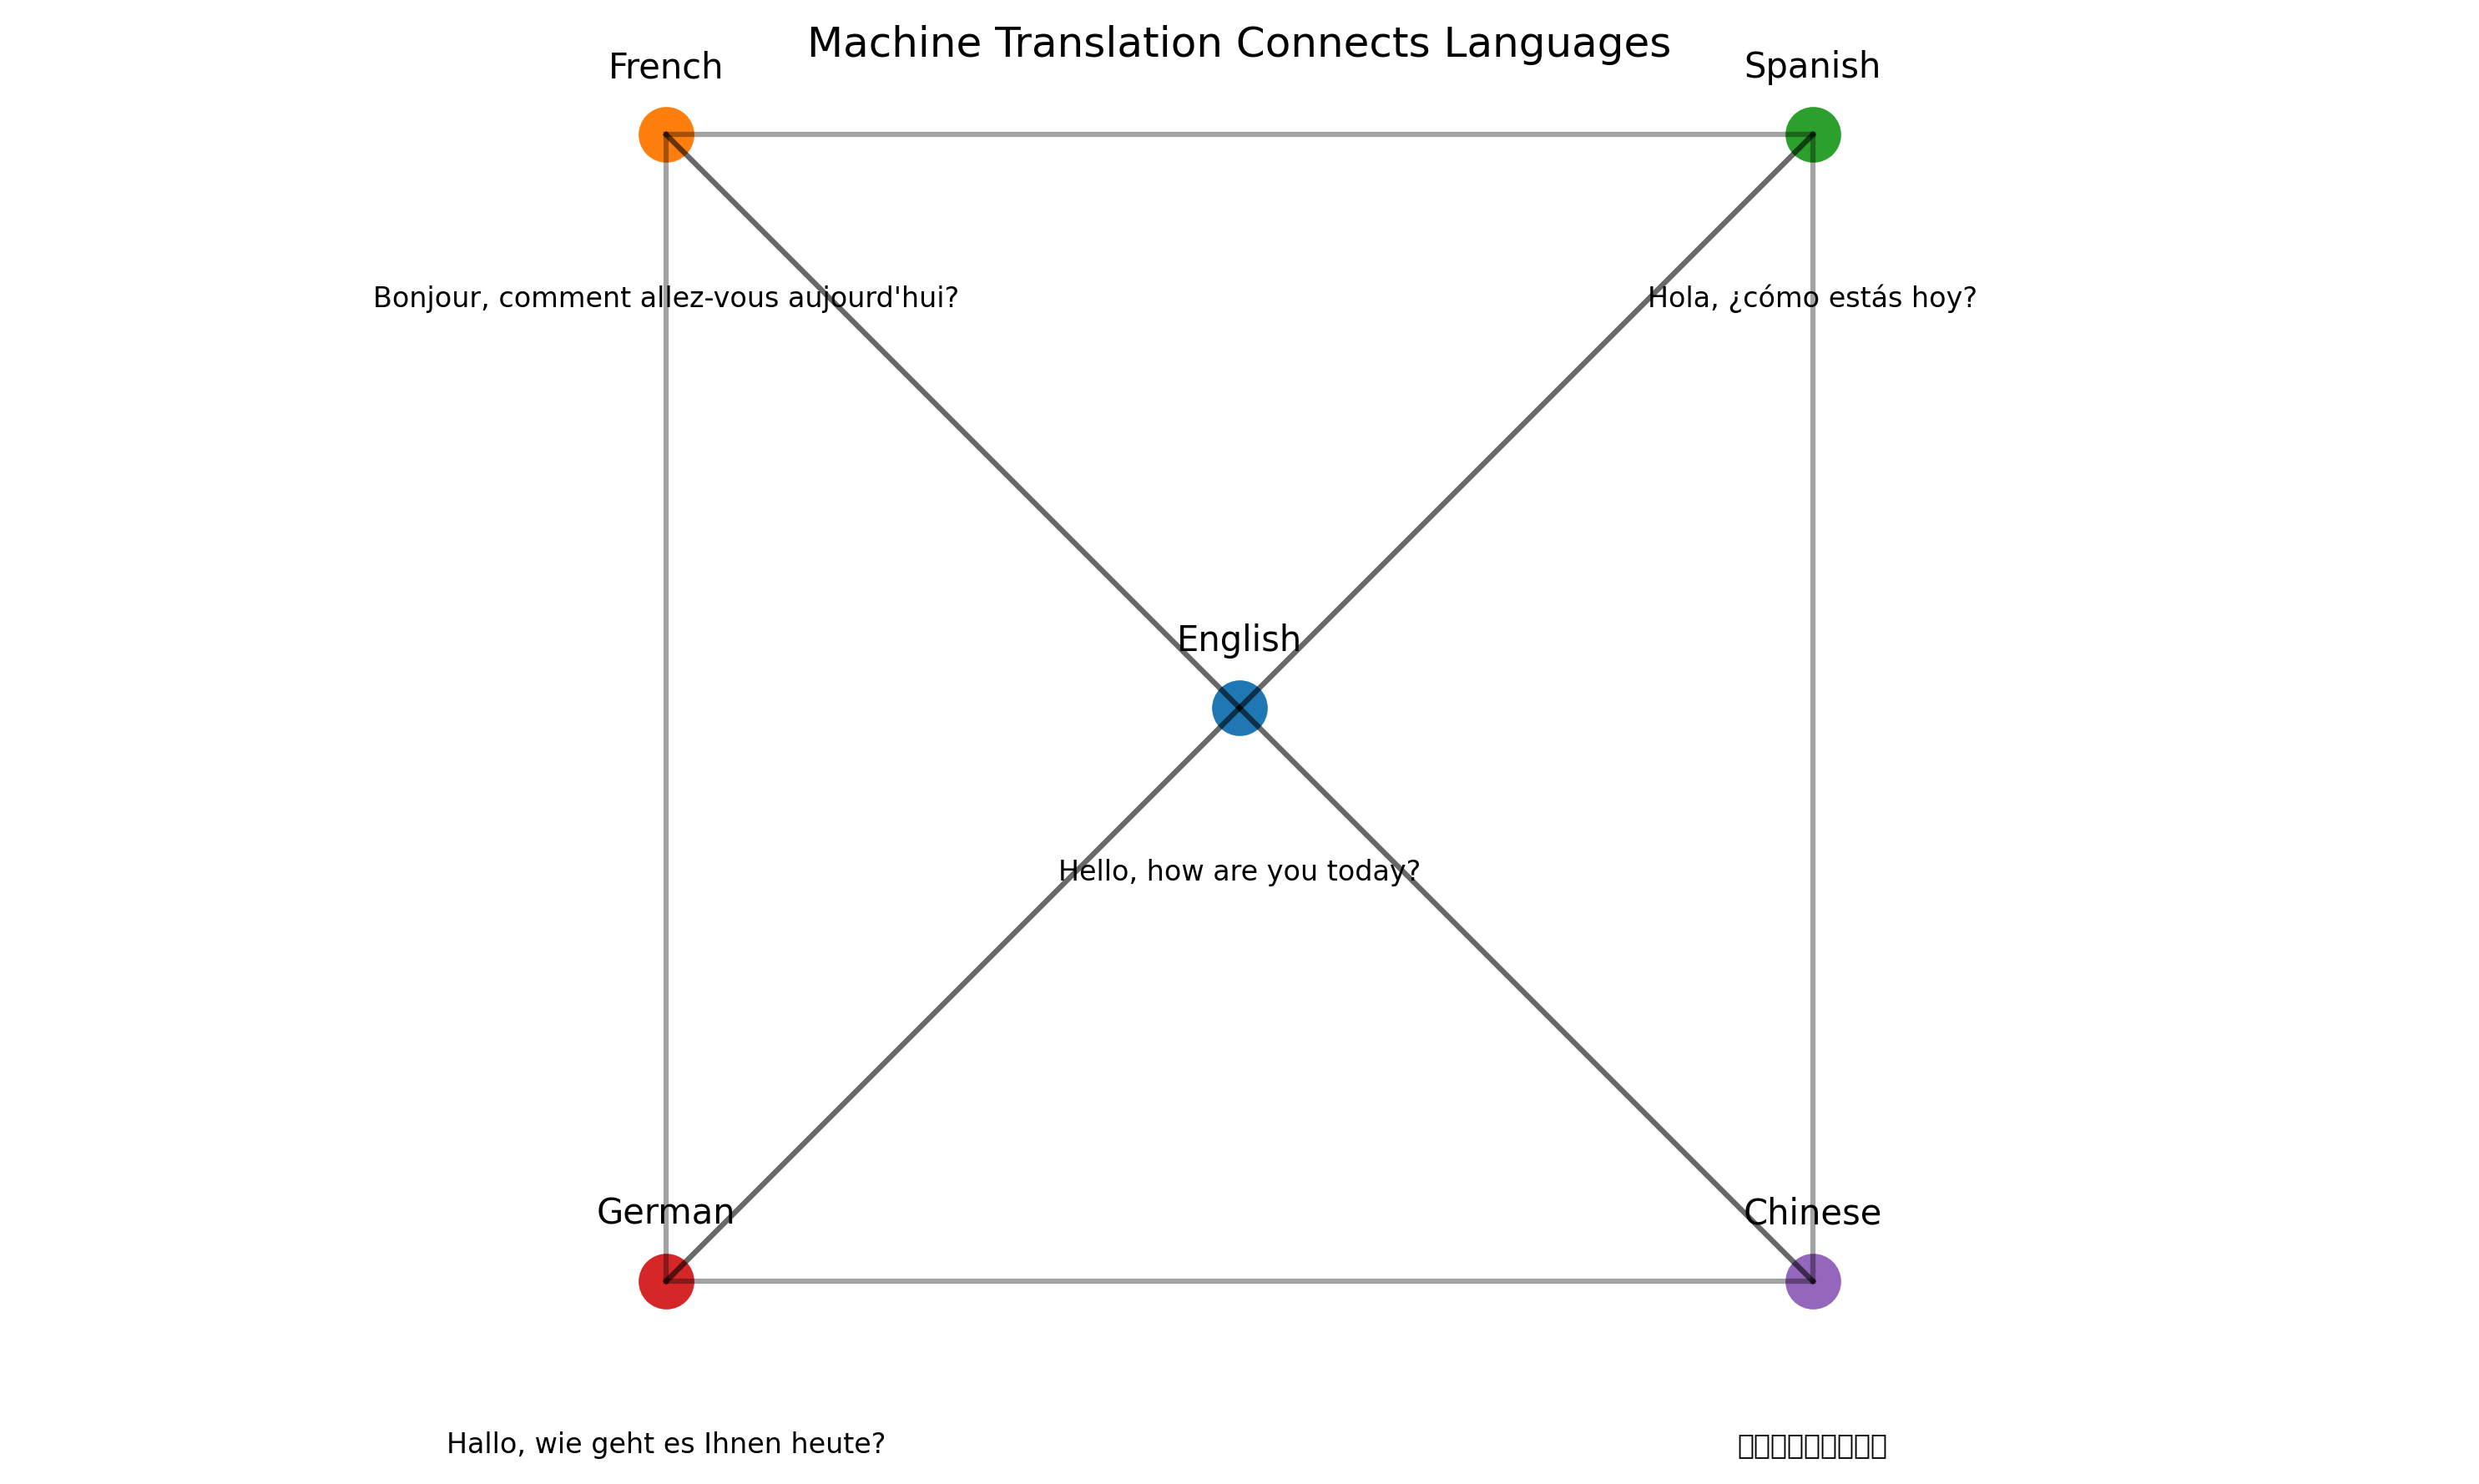
\includegraphics[width=\textwidth]{images/generated/translation.png}
        \end{column}
        \begin{column}{0.5\textwidth}
            \textbf{Chatbots et assistants virtuels}
            \begin{itemize}
                \item Répondent automatiquement aux questions
                \item Peuvent effectuer des tâches spécifiques
                \item Applications: assistants vocaux, service client
            \end{itemize}
            \vspace{0.3cm}
            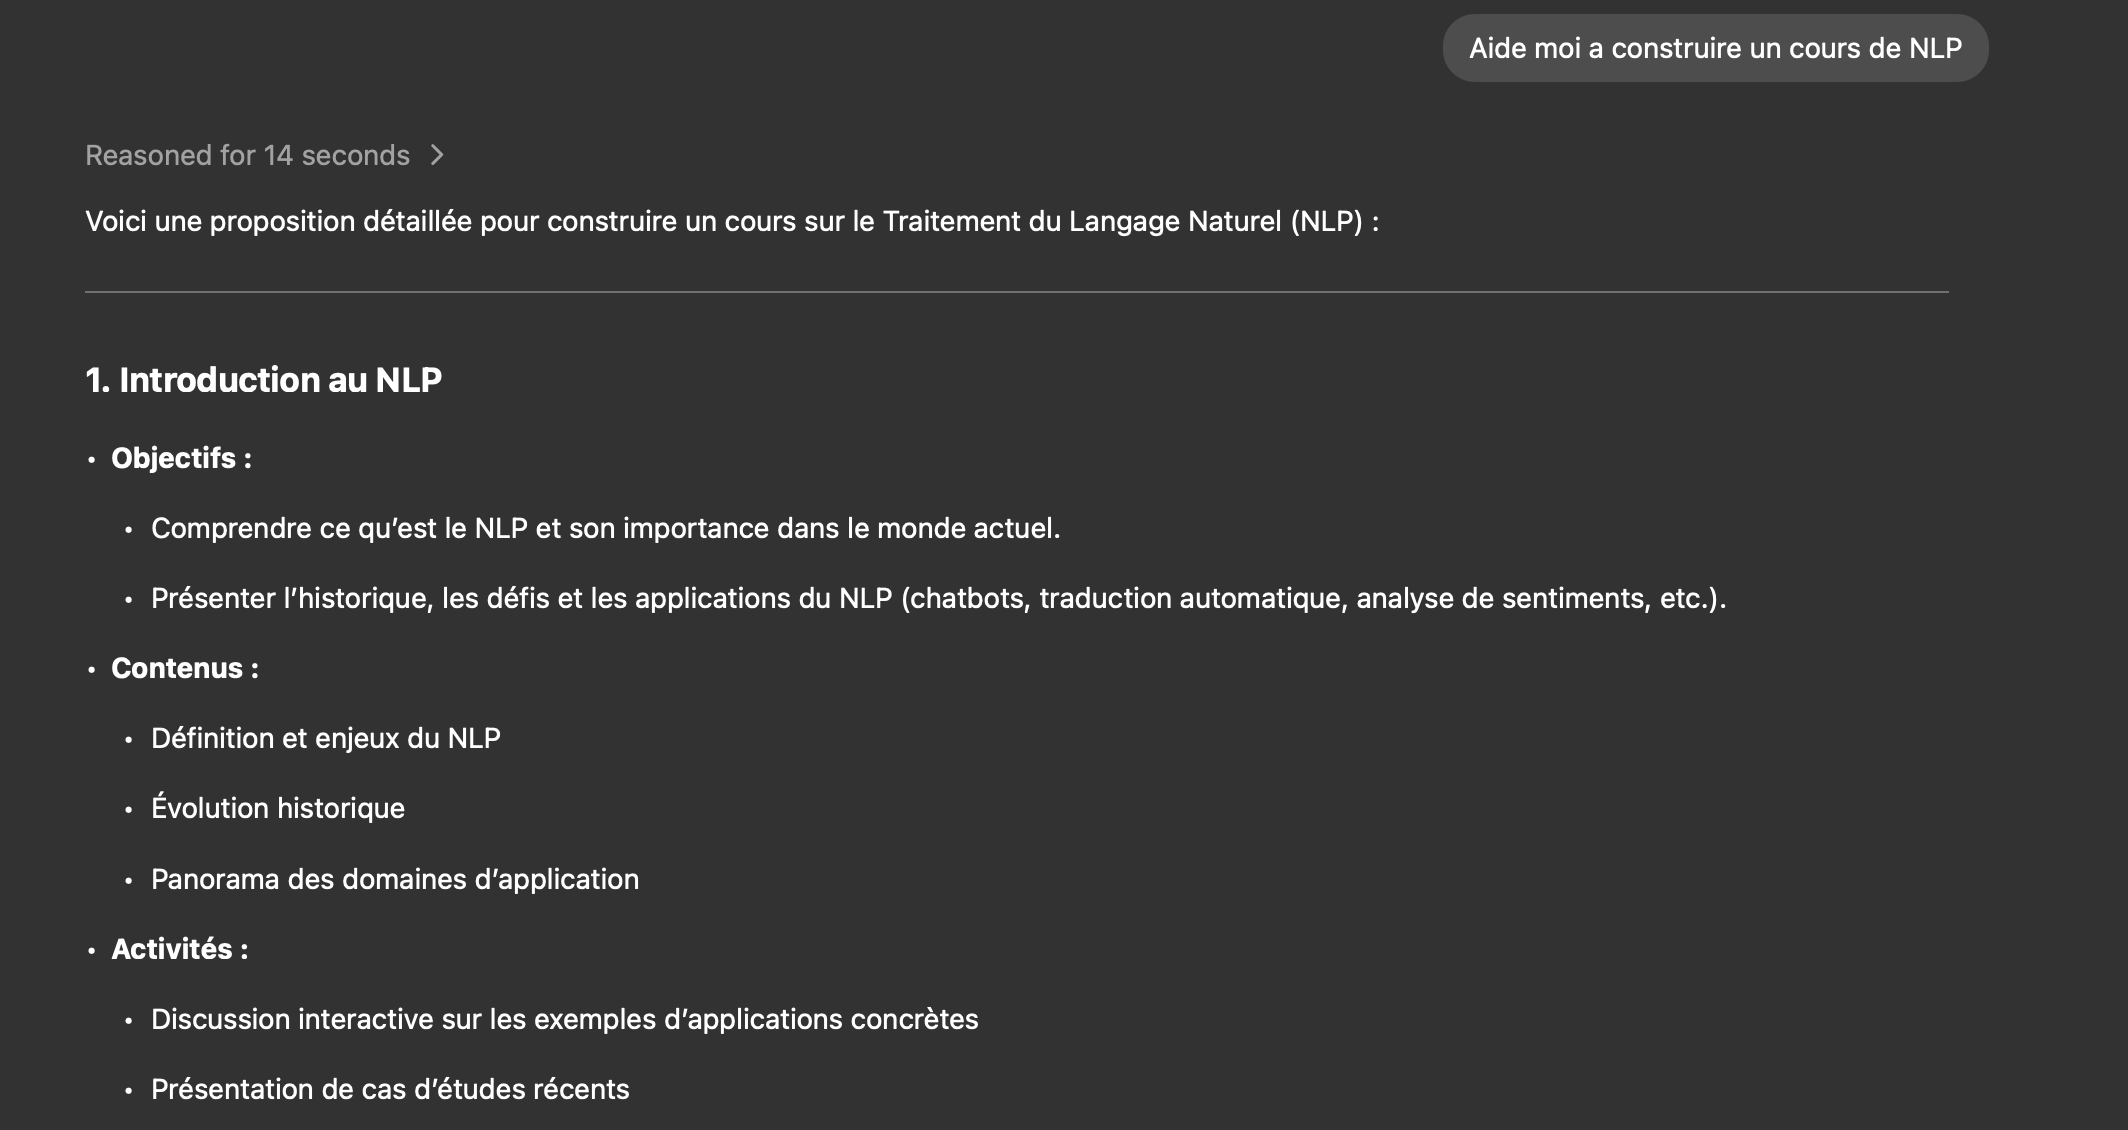
\includegraphics[width=\textwidth]{images/chatbot.png}
        \end{column}
    \end{columns}
\end{frame}

% New section on NLP basics and tokenization
\section{Bases du Traitement du Langage Naturel}

% Slide: What is a word in computing
\begin{frame}{Représentation des mots en informatique}
    \begin{itemize}
        \item En informatique, un \textbf{mot} est représenté comme une \textbf{séquence de caractères}
        \item Chaque \textbf{caractère} est encodé sur un nombre fini de bits:
        \begin{itemize}
            \item ASCII: 7 bits (128 caractères)
            \item Unicode: jusqu'à 32 bits (plus de 143 000 caractères)
        \end{itemize}
        \vspace{0.3cm}
        \item Pour traiter le langage, les modèles ont besoin de \textbf{représentations numériques}
        \item Le texte doit être converti en nombres pour être compris par les algorithmes
        \item Cette conversion s'appelle la \textbf{tokenisation}
        \vspace{0.3cm}
        \item \textbf{Exemple}: "L'intelligence artificielle transforme notre monde."
        \begin{itemize}
            \item Comment représenter cette phrase pour un modèle?
        \end{itemize}
    \end{itemize}
\end{frame}

% Slide: Different tokenization methods - Character tokenization
\begin{frame}{Encodage des caractères}
    \begin{columns}
        \begin{column}{0.55\textwidth}
            \begin{itemize}
                \item En informatique, chaque caractère a un \textbf{identifiant numérique unique}
                \begin{itemize}
                    \item Exemple simple: a=0, b=1, c=2, etc.
                    \item En réalité: tables d'encodage (ASCII, Unicode)
                \end{itemize}
                \vspace{0.1cm}
                \item \textbf{Tokenisation par caractère}:
                \begin{itemize}
                    \item Chaque caractère = un token
                    \item Vocabulaire très limité (128-256 tokens)
                    \item Séquences très longues
                \end{itemize}
                \vspace{0.1cm}
                \item \textbf{Avantages}:
                \begin{itemize}
                    \item Pas de mots inconnus
                    \item Solution universelle pour toutes les langues
                \end{itemize}
            \end{itemize}
        \end{column}
        \begin{column}{0.45\textwidth}
            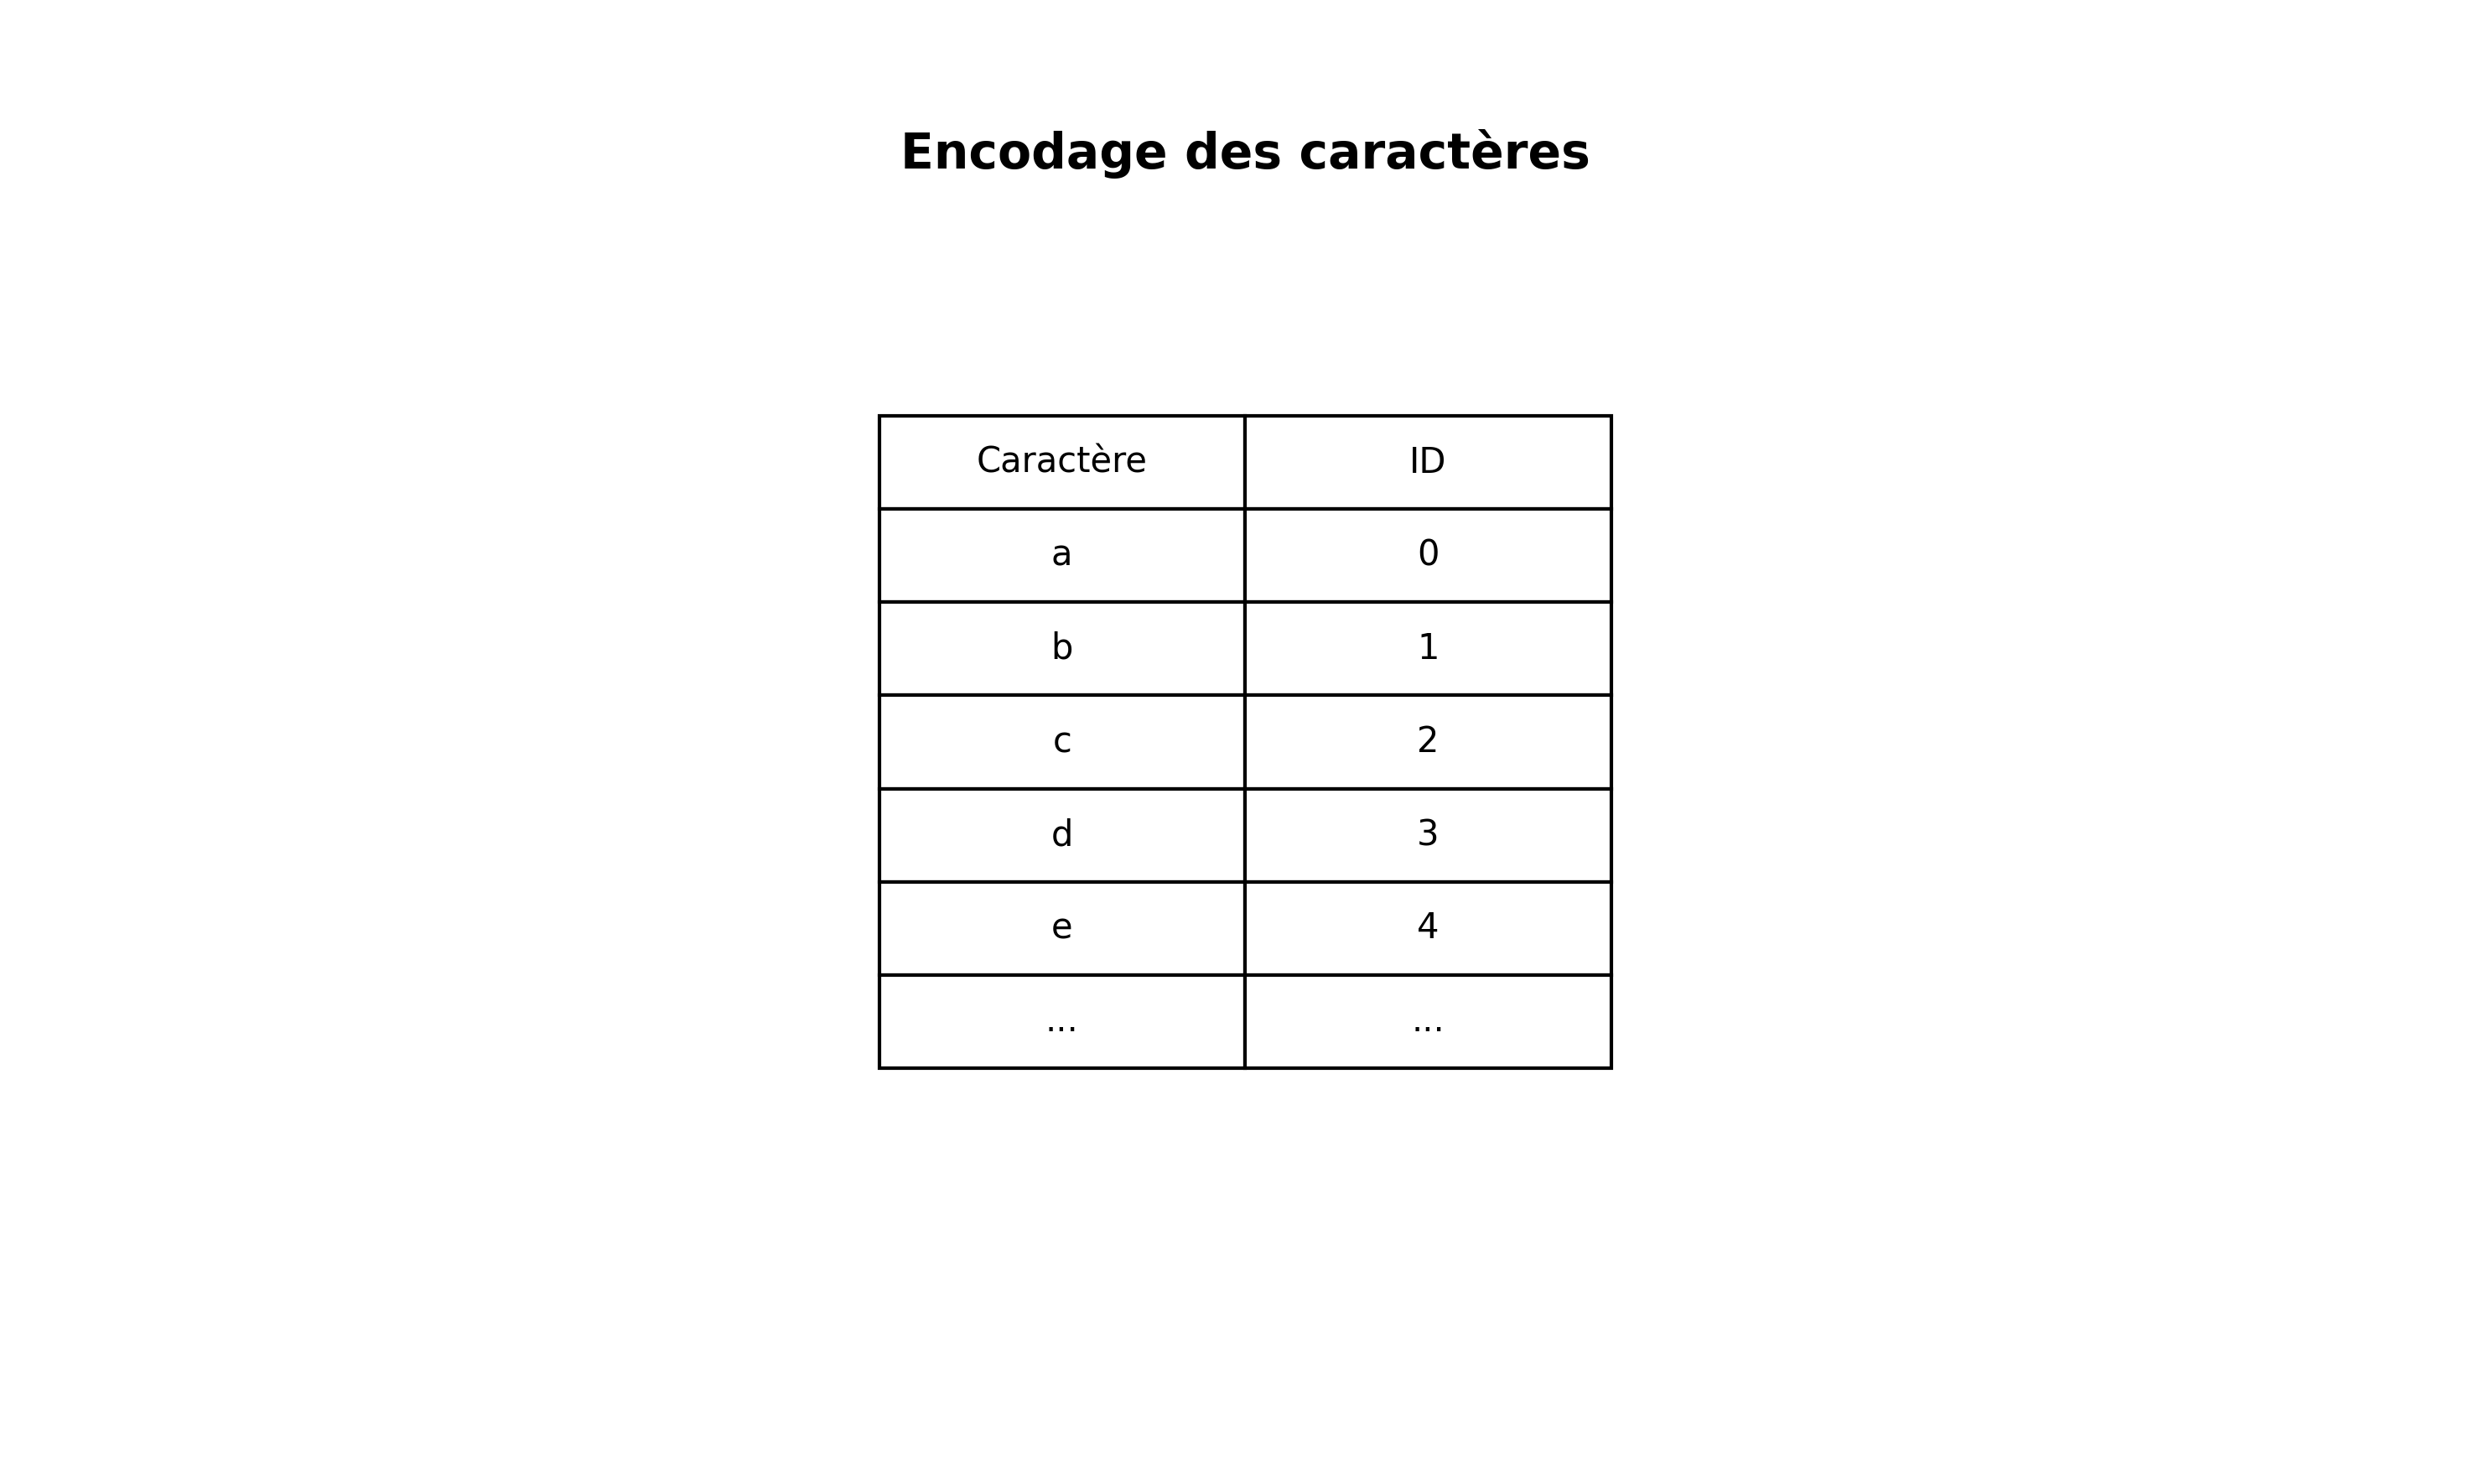
\includegraphics[width=0.95\textwidth]{images/generated/char_tokenization.png}
            \vspace{0.1cm}
            \begin{center}
                \small{Correspondance entre caractères et identifiants}
            \end{center}
        \end{column}
    \end{columns}
\end{frame}

% Slide: Different tokenization methods - Word and subword tokenization
\begin{frame}{Méthodes de tokenisation 2: Mots et sous-mots}
    \begin{columns}
        \begin{column}{0.5\textwidth}
            \begin{itemize}
                \item \textbf{Tokenisation par mot}:
                \begin{itemize}
                    \item Chaque mot = un token
                    \item Vocabulaire très grand (100K-1M tokens)
                    \item Problème des mots inconnus (OOV)
                    \item Difficulté avec les variations morphologiques
                \end{itemize}
                \vspace{0.3cm}
                \item \textbf{Tokenisation par sous-mots}:
                \begin{itemize}
                    \item Compromis entre caractères et mots
                    \item Vocabulaire raisonnable (10K-50K tokens)
                    \item Capture les morphèmes et parties de mots
                    \item Solution privilégiée par les modèles actuels
                \end{itemize}
            \end{itemize}
        \end{column}
        \begin{column}{0.5\textwidth}
            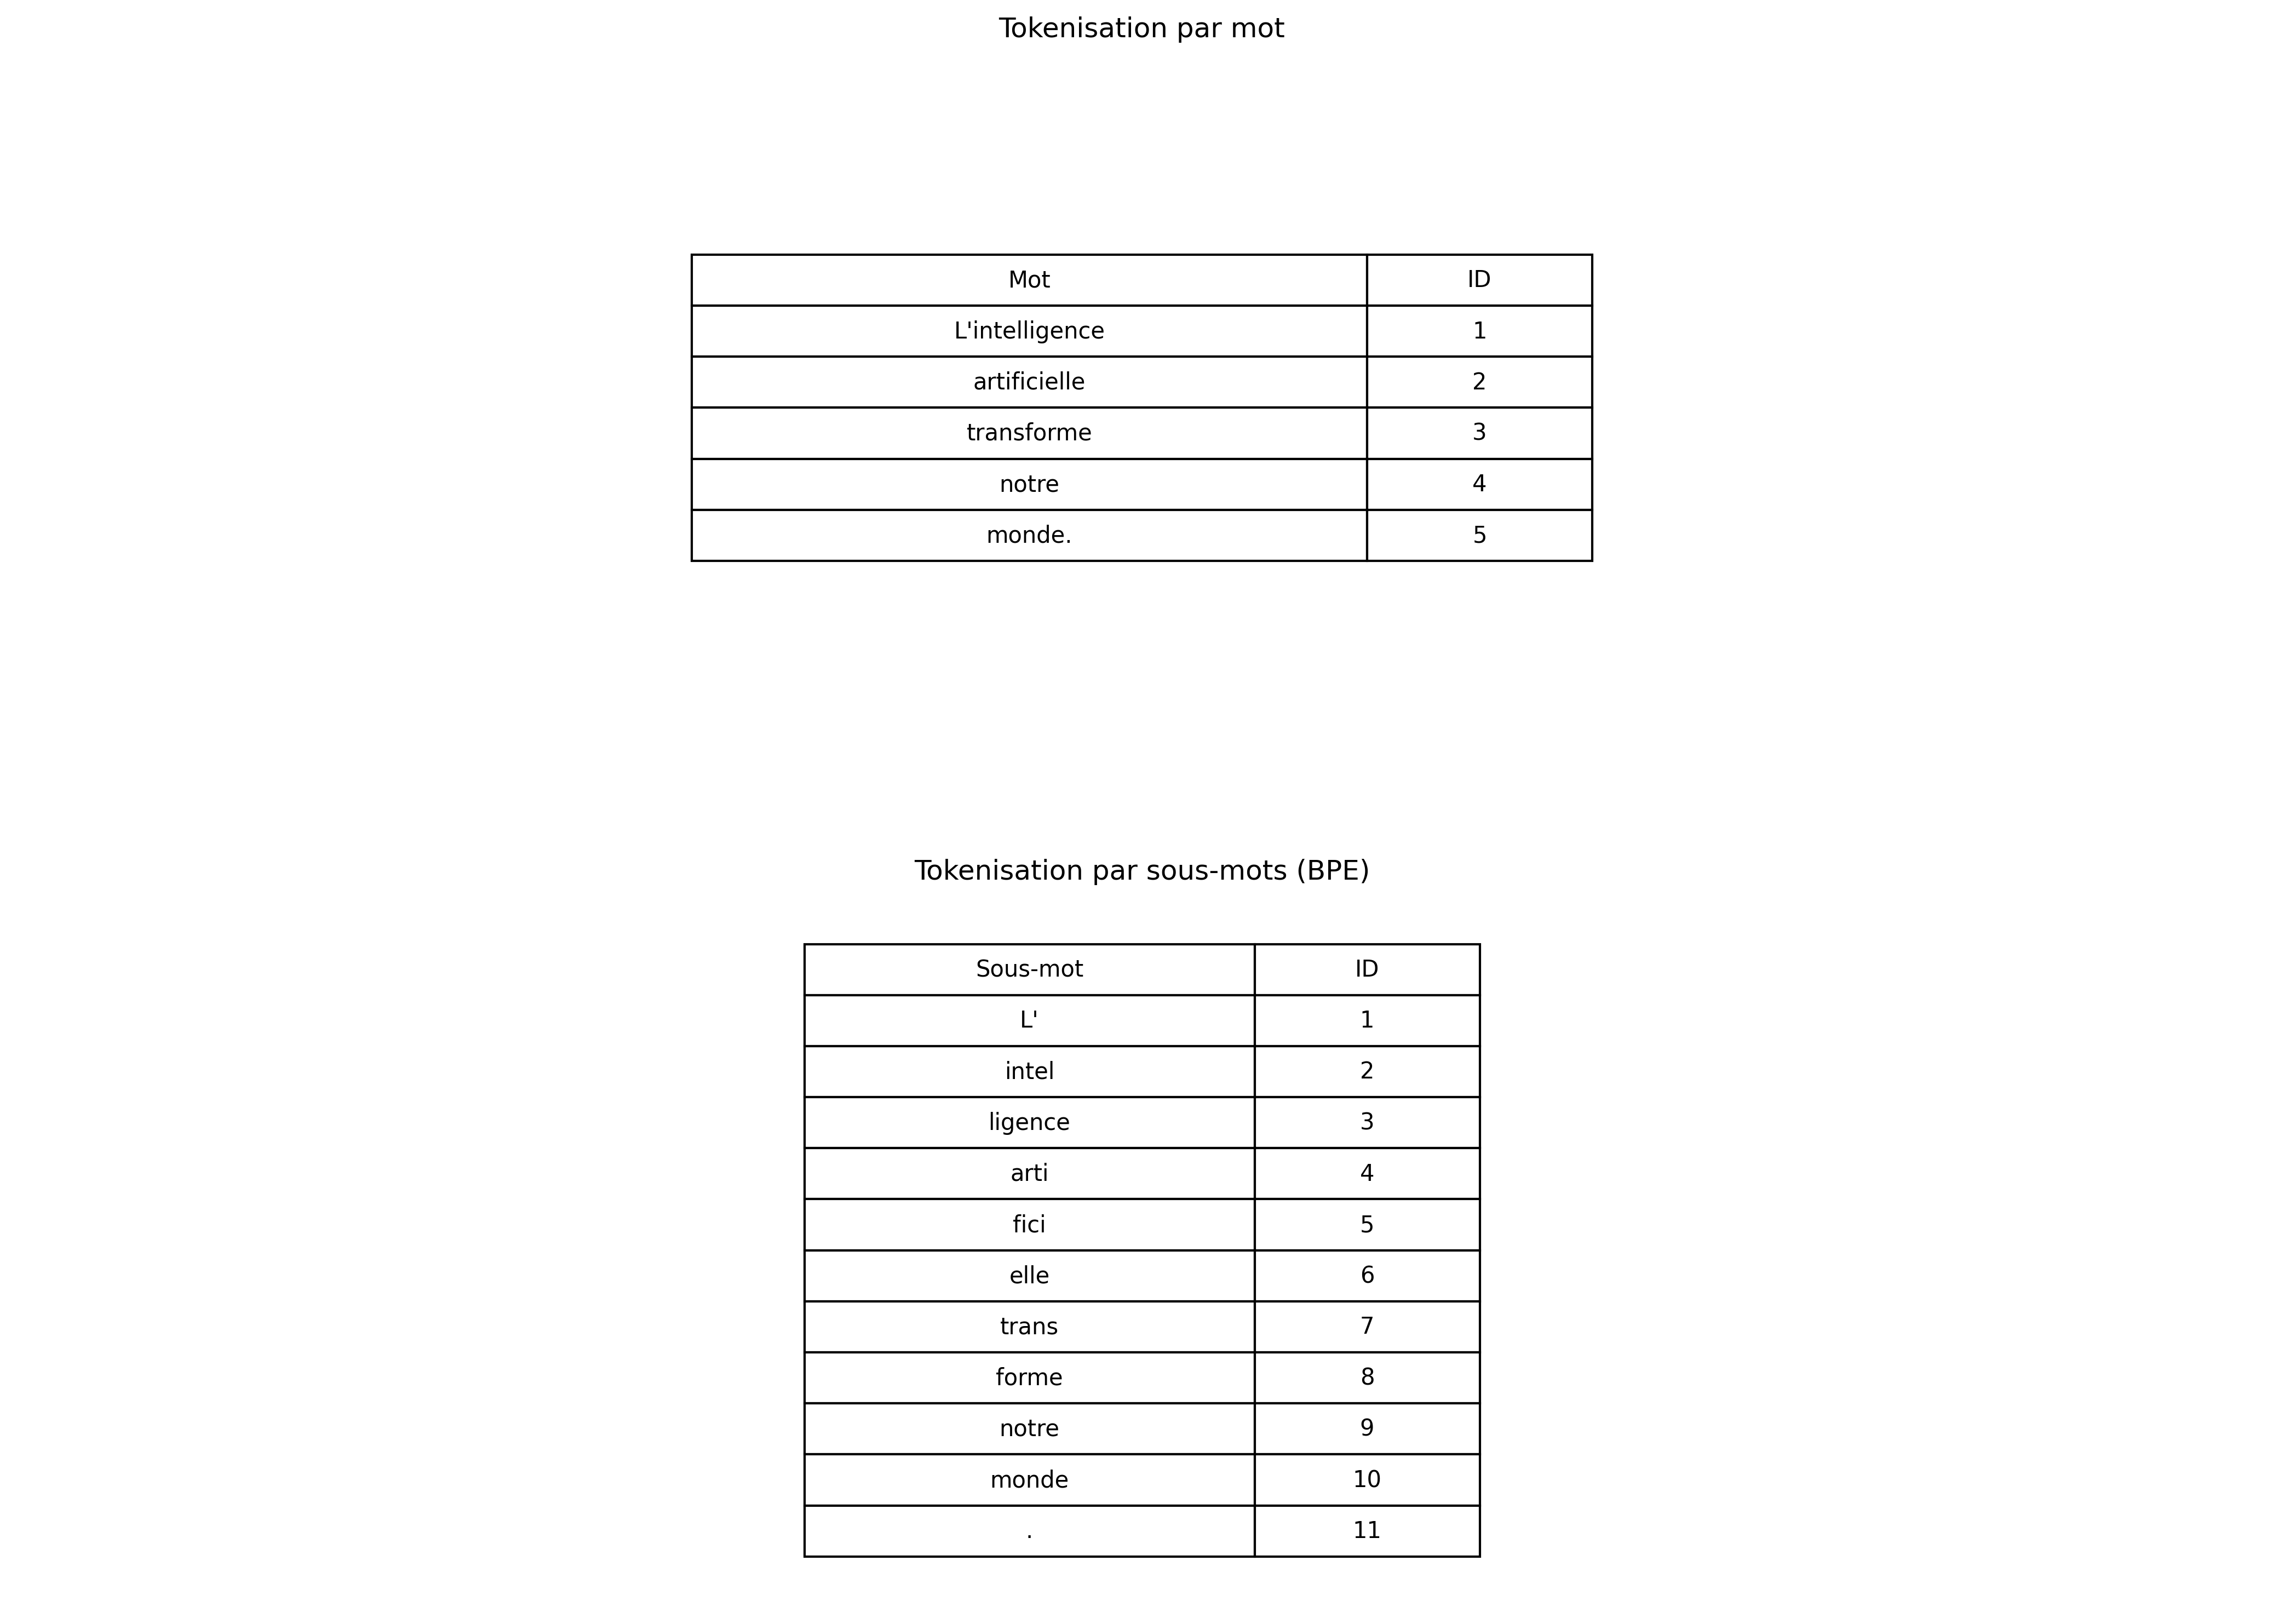
\includegraphics[width=\textwidth]{images/generated/word_subword_tokenization.png}
            \vspace{0.2cm}
            \begin{center}
                \small{Tokenisations par mot et sous-mot de la phrase d'exemple}
            \end{center}
        \end{column}
    \end{columns}
\end{frame}

% Slide: Vocabulary size comparison
\begin{frame}{Comparaison des tailles de vocabulaire}
    \begin{columns}
        \begin{column}{0.5\textwidth}
            \textbf{Compromis entre taille et expressivité}:
            \begin{itemize}
                \item \textbf{Vocabulaire petit} (caractères):
                \begin{itemize}
                    \item Avantage: pas de mots inconnus
                    \item Inconvénient: séquences très longues
                \end{itemize}
                \vspace{0.3cm}
                \item \textbf{Vocabulaire grand} (mots):
                \begin{itemize}
                    \item Avantage: capture directement les unités sémantiques
                    \item Inconvénient: nombreux mots inconnus
                \end{itemize}
                \vspace{0.3cm}
                \item \textbf{Vocabulaire intermédiaire} (sous-mots):
                \begin{itemize}
                    \item Équilibre entre les deux approches
                    \item Solution adoptée par la plupart des modèles modernes
                \end{itemize}
            \end{itemize}
        \end{column}
        \begin{column}{0.5\textwidth}
            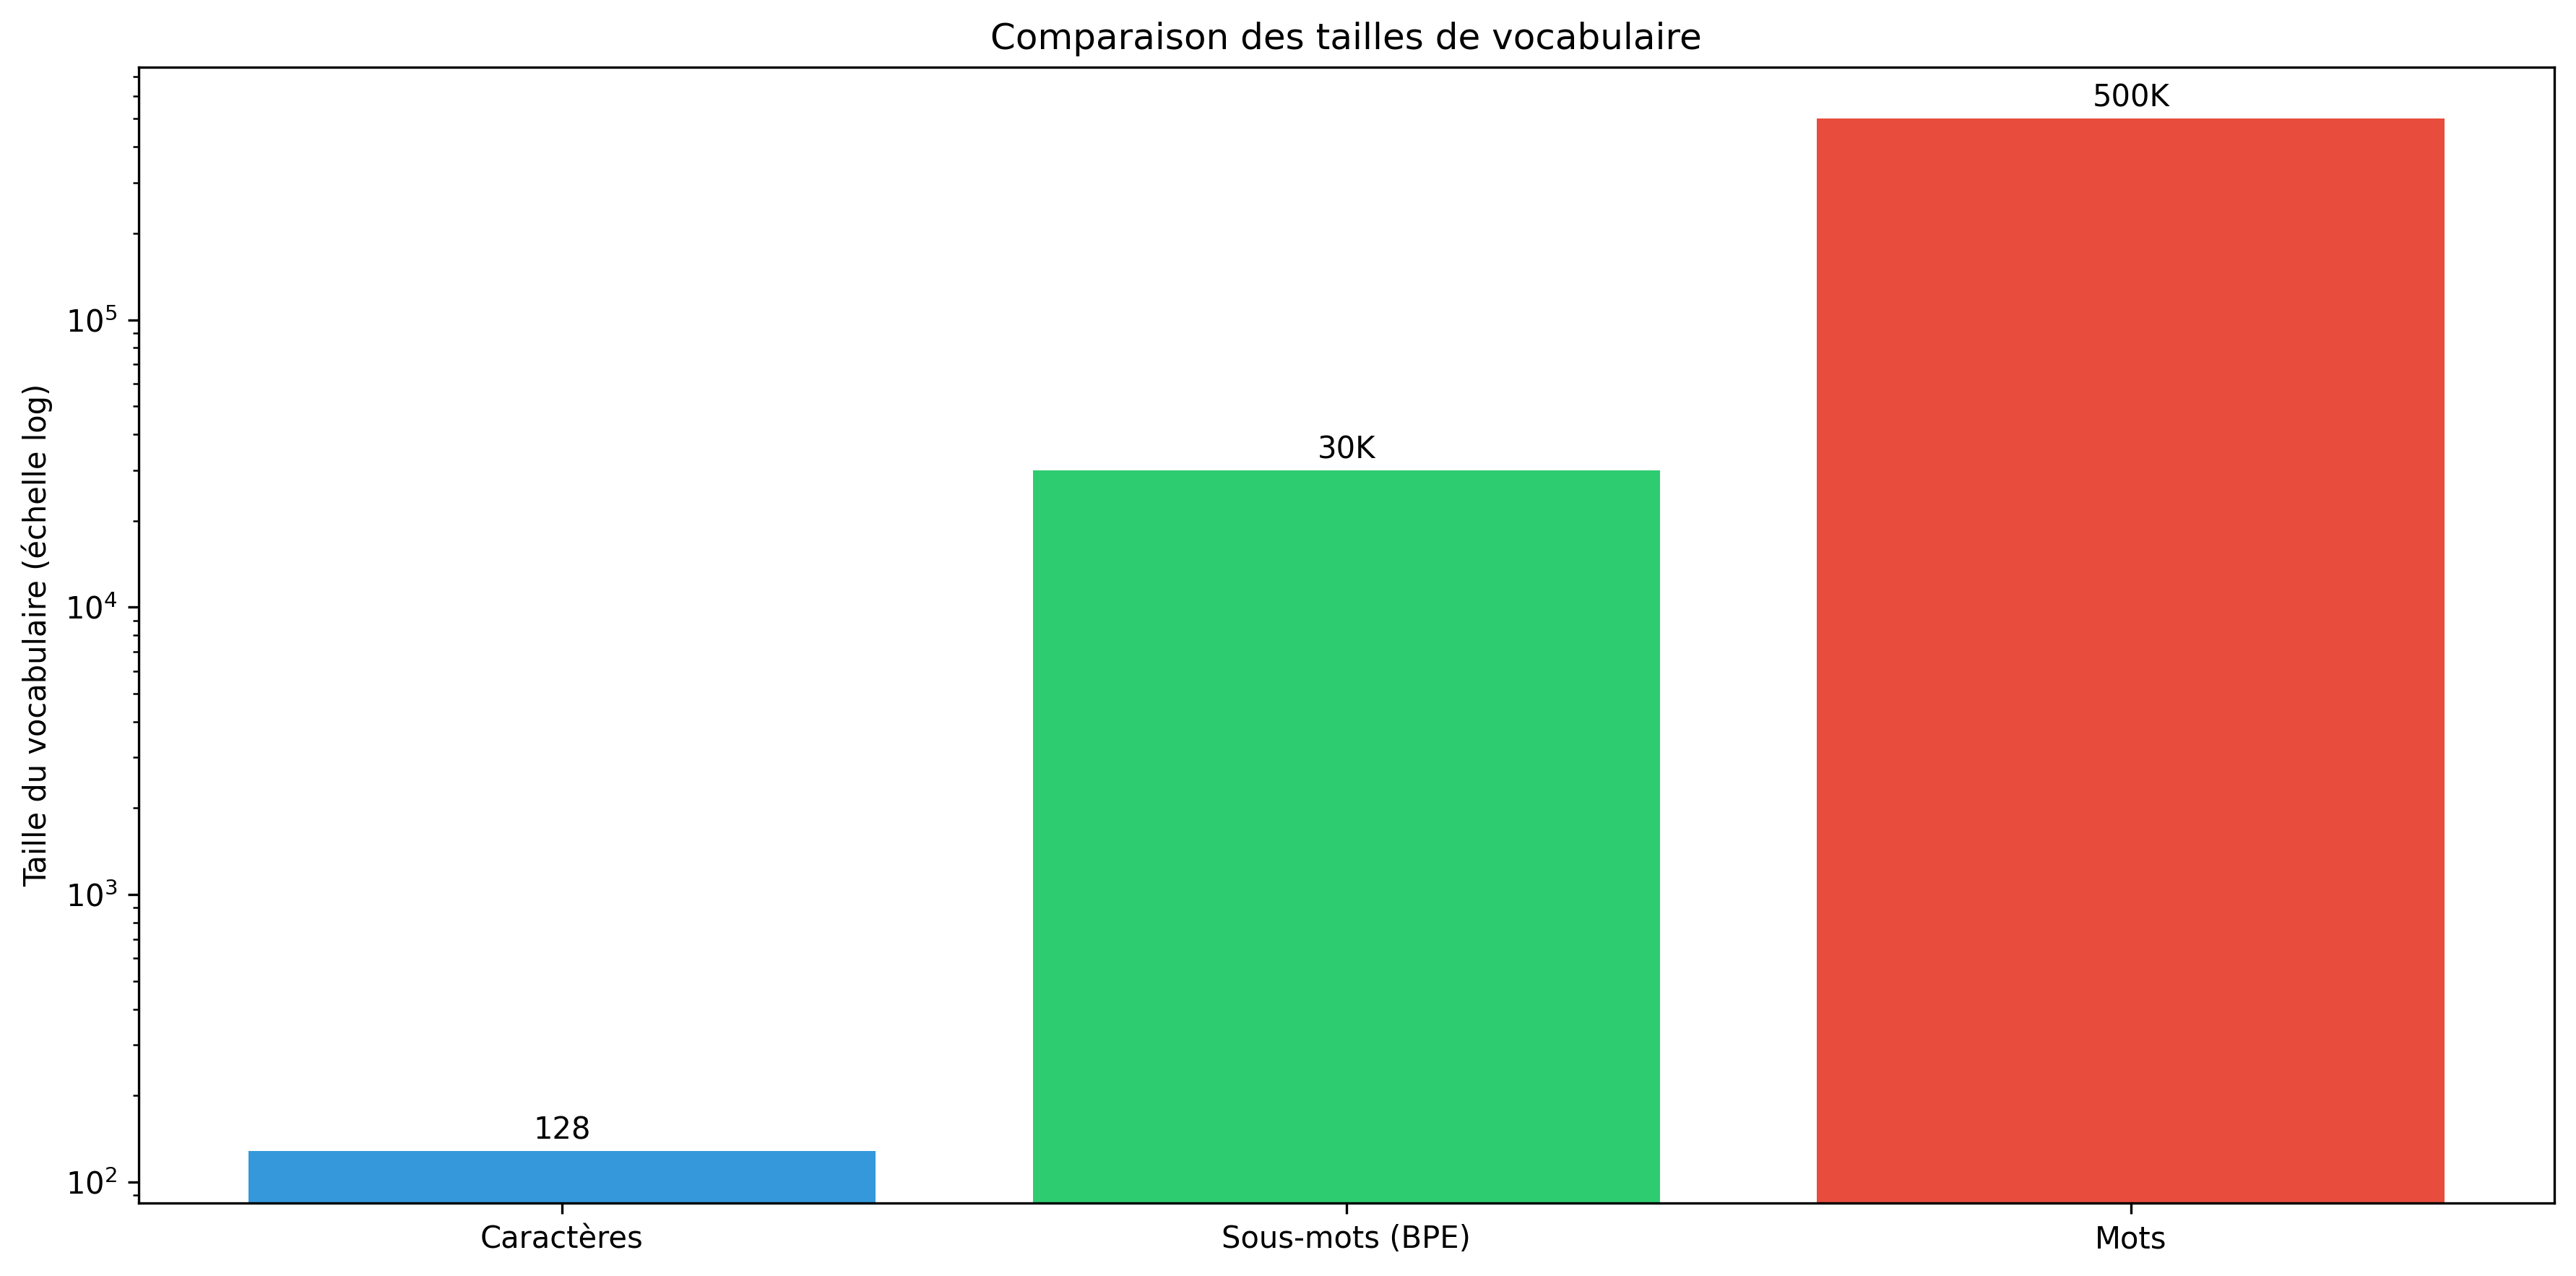
\includegraphics[width=\textwidth]{images/generated/vocab_size_comparison.png}
            \vspace{0.2cm}
            \begin{center}
                \small{Comparaison des tailles de vocabulaire selon la méthode}
            \end{center}
        \end{column}
    \end{columns}
\end{frame}

% Slide: BPE Algorithm
\begin{frame}{Algorithme BPE (Byte Pair Encoding)}
    \begin{columns}
        \begin{column}{0.45\textwidth}
            \textbf{Principe du BPE}:
            \begin{enumerate}
                \item Commencer avec un vocabulaire de caractères
                \item Identifier les paires de tokens les plus fréquentes
                \item Fusionner ces paires pour créer un nouveau token
                \item Répéter jusqu'à atteindre la taille de vocabulaire souhaitée
            \end{enumerate}
            \vspace{0.3cm}
            \textbf{Avantages}:
            \begin{itemize}
                \item Adapté au corpus d'entraînement
                \item Gère efficacement les mots rares
                \item Capture les morphèmes et affixes
                \item Utilisé dans GPT, BERT, T5, etc.
            \end{itemize}
        \end{column}
        \begin{column}{0.55\textwidth}
            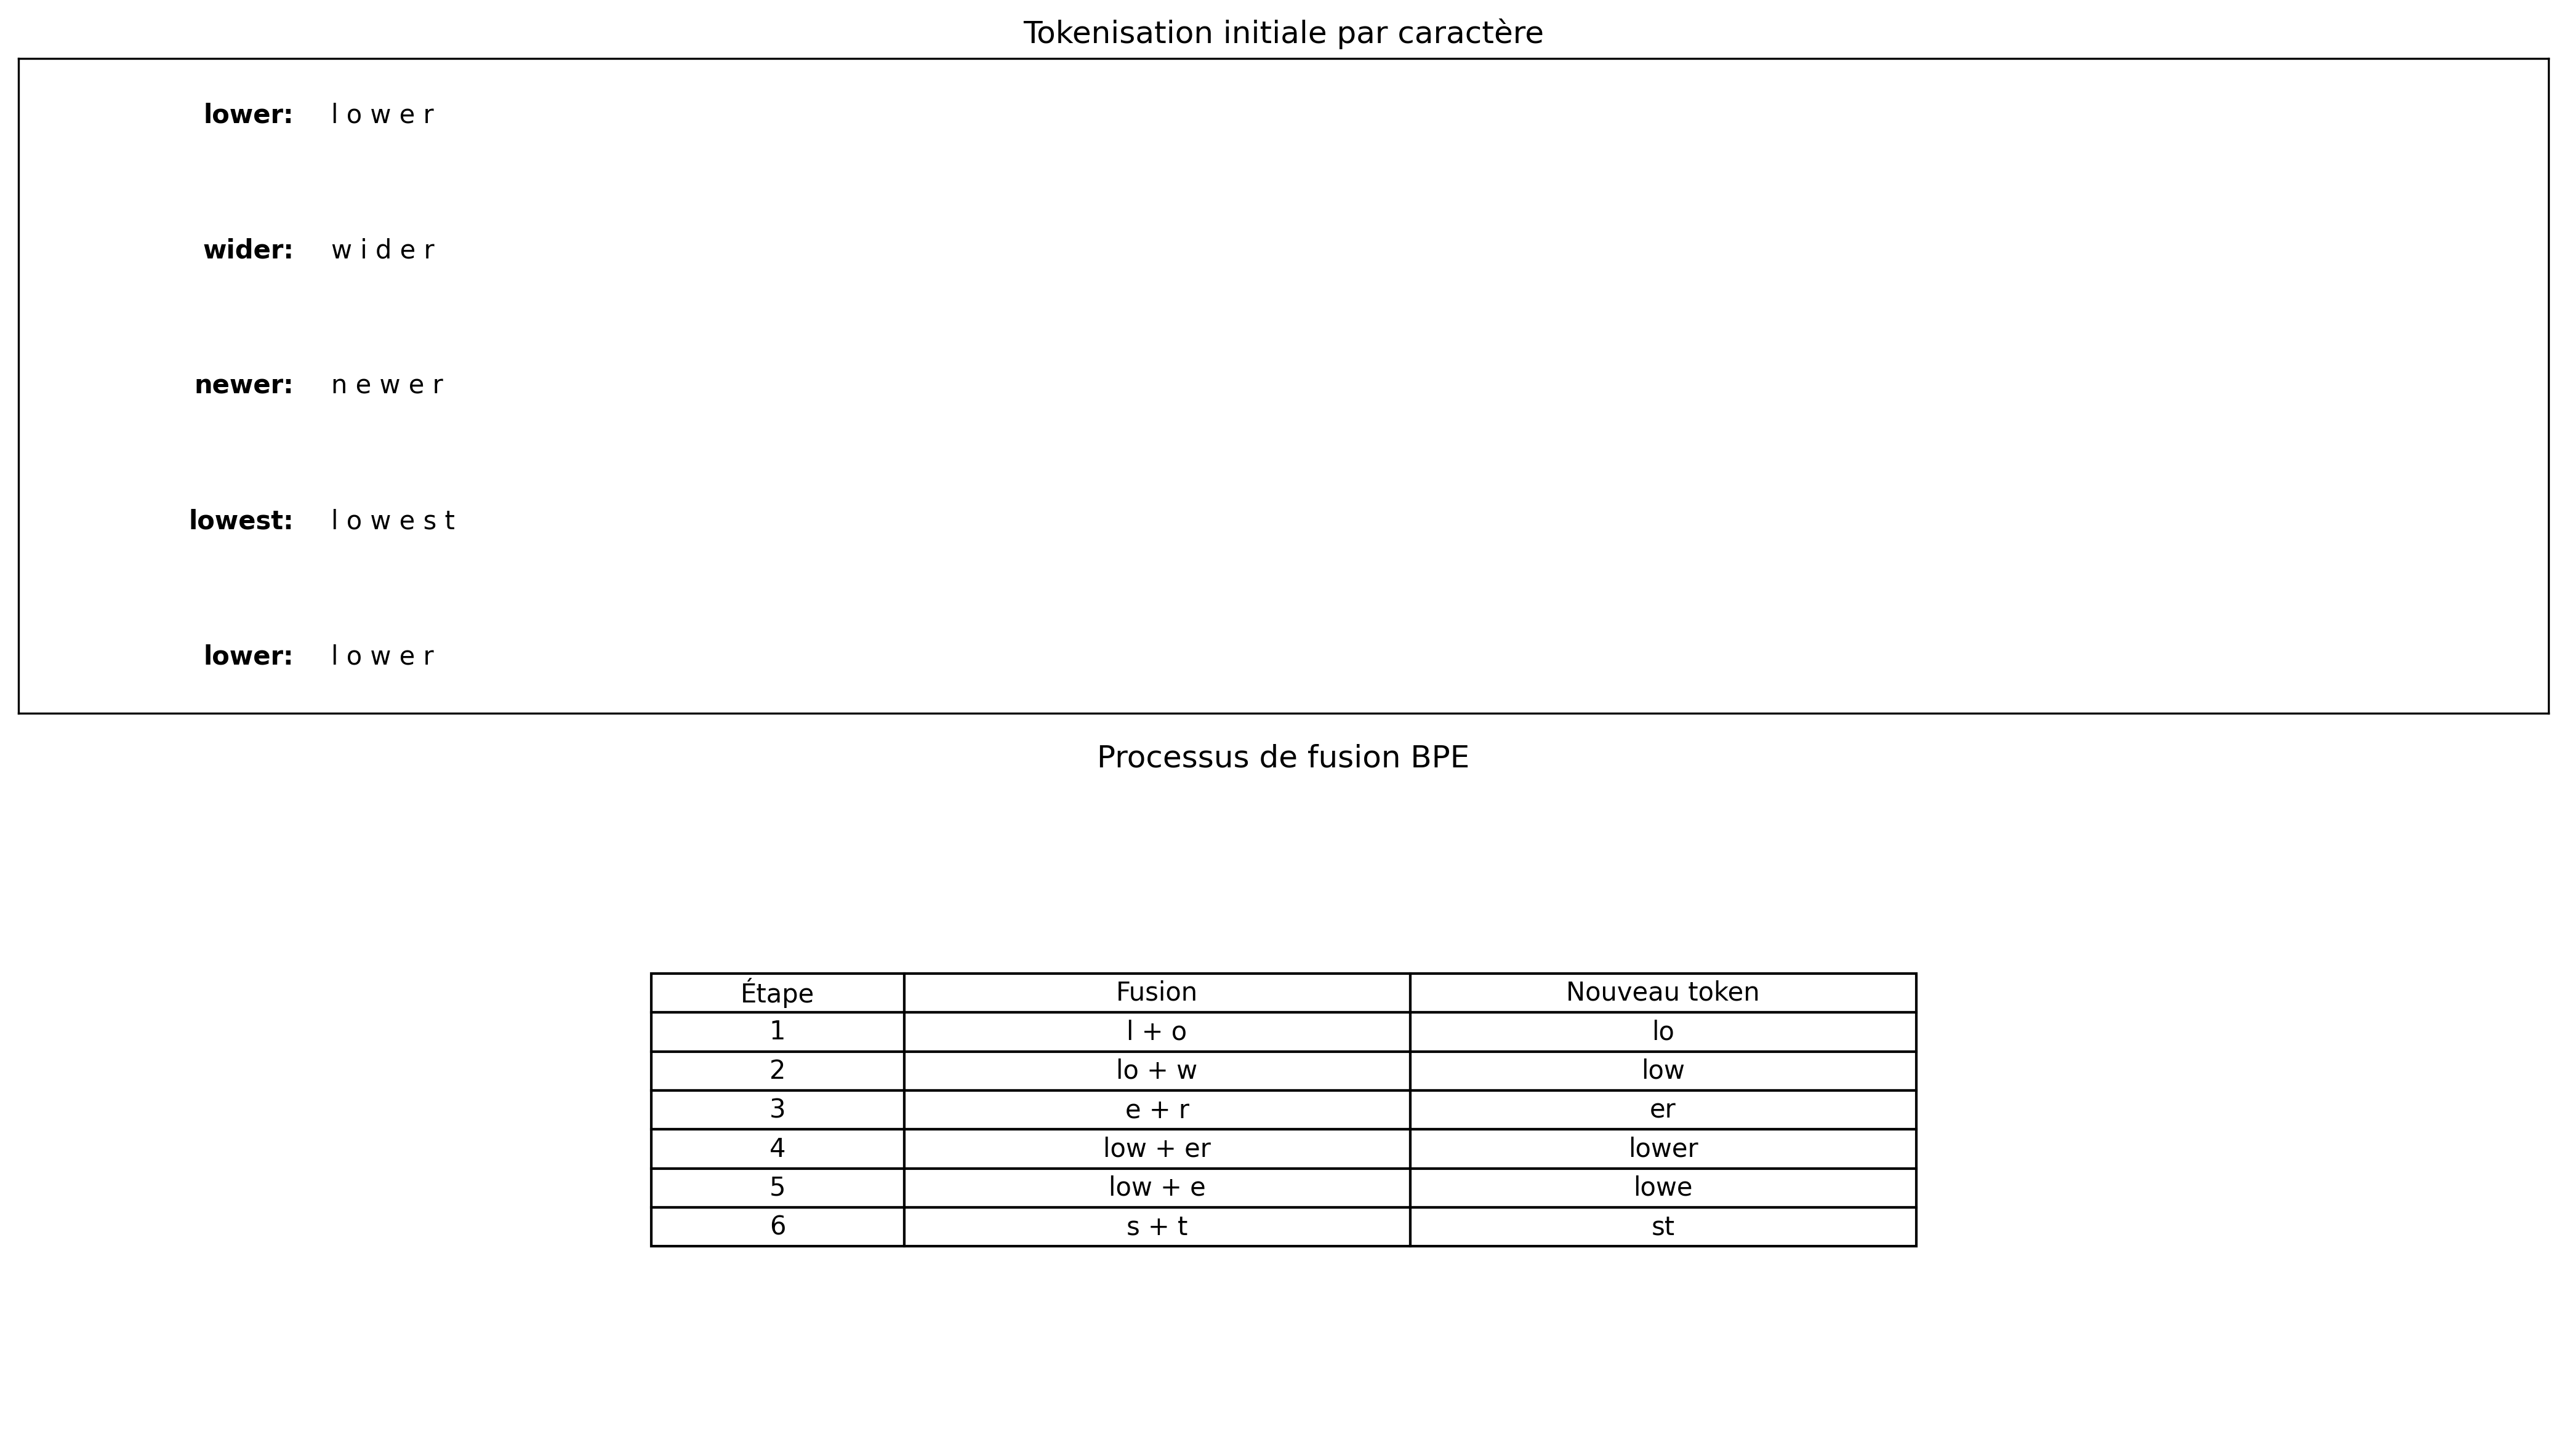
\includegraphics[width=\textwidth]{images/generated/bpe_algorithm.png}
            \vspace{0.2cm}
            \begin{center}
                \small{Exemple de fusion progressive avec BPE}
            \end{center}
        \end{column}
    \end{columns}
\end{frame}

% New section on the future of LLMs
\section{Le Futur des Modèles de Langage (LLMs)}

% Slide: Introduction to LLMs and their evolution
\begin{frame}{Évolution des Modèles de Langage à Grande Échelle}
    \begin{itemize}
        \item Les \textbf{Large Language Models (LLMs)} représentent une avancée majeure en NLP
        \item \textbf{Évolution rapide} depuis 2018:
        \begin{itemize}
            \item GPT-1 (0.1B paramètres) $\rightarrow$ GPT-4 ($>$1T paramètres estimés)
            \item Augmentation de la taille des modèles = capacités émergentes
        \end{itemize}
        \item \textbf{Capacités actuelles}:
        \begin{itemize}
            \item Génération de texte cohérent et contextuel
            \item Adaptation à différentes tâches sans fine-tuning spécifique
            \item Compréhension complexe et résolution de problèmes
            \item Génération de code, traduction avancée, créativité
        \end{itemize}
        \item Ces modèles transforment comment nous \textbf{interagissons avec l'information} et \textbf{automatisons les tâches cognitives}
    \end{itemize}
\end{frame}

% Slide: Advanced reasoning capabilities of LLMs
\begin{frame}{Capacités de Raisonnement Avancées}
    \begin{columns}
        \begin{column}{0.55\textwidth}
            \textbf{Émergence du raisonnement complexe}
            \begin{itemize}
                \item \textbf{Test-Time Scaling}: Amélioration des performances avec plus de temps d'inférence
                \begin{itemize}
                    \item Chain-of-Thought (CoT): raisonnement étape par étape
                    \item Tree-of-Thoughts (ToT): exploration de multiples voies de raisonnement
                    \item Self-consistency: génération de plusieurs solutions et vote majoritaire
                \end{itemize}
                \vspace{0.3cm}
                \item \textbf{Émergence avec l'échelle}
                \begin{itemize}
                    \item Les capacités émergent non-linéairement avec la taille du modèle
                    \item Point critique où le raisonnement "apparaît"
                \end{itemize}
            \end{itemize}
        \end{column}
        \begin{column}{0.45\textwidth}
            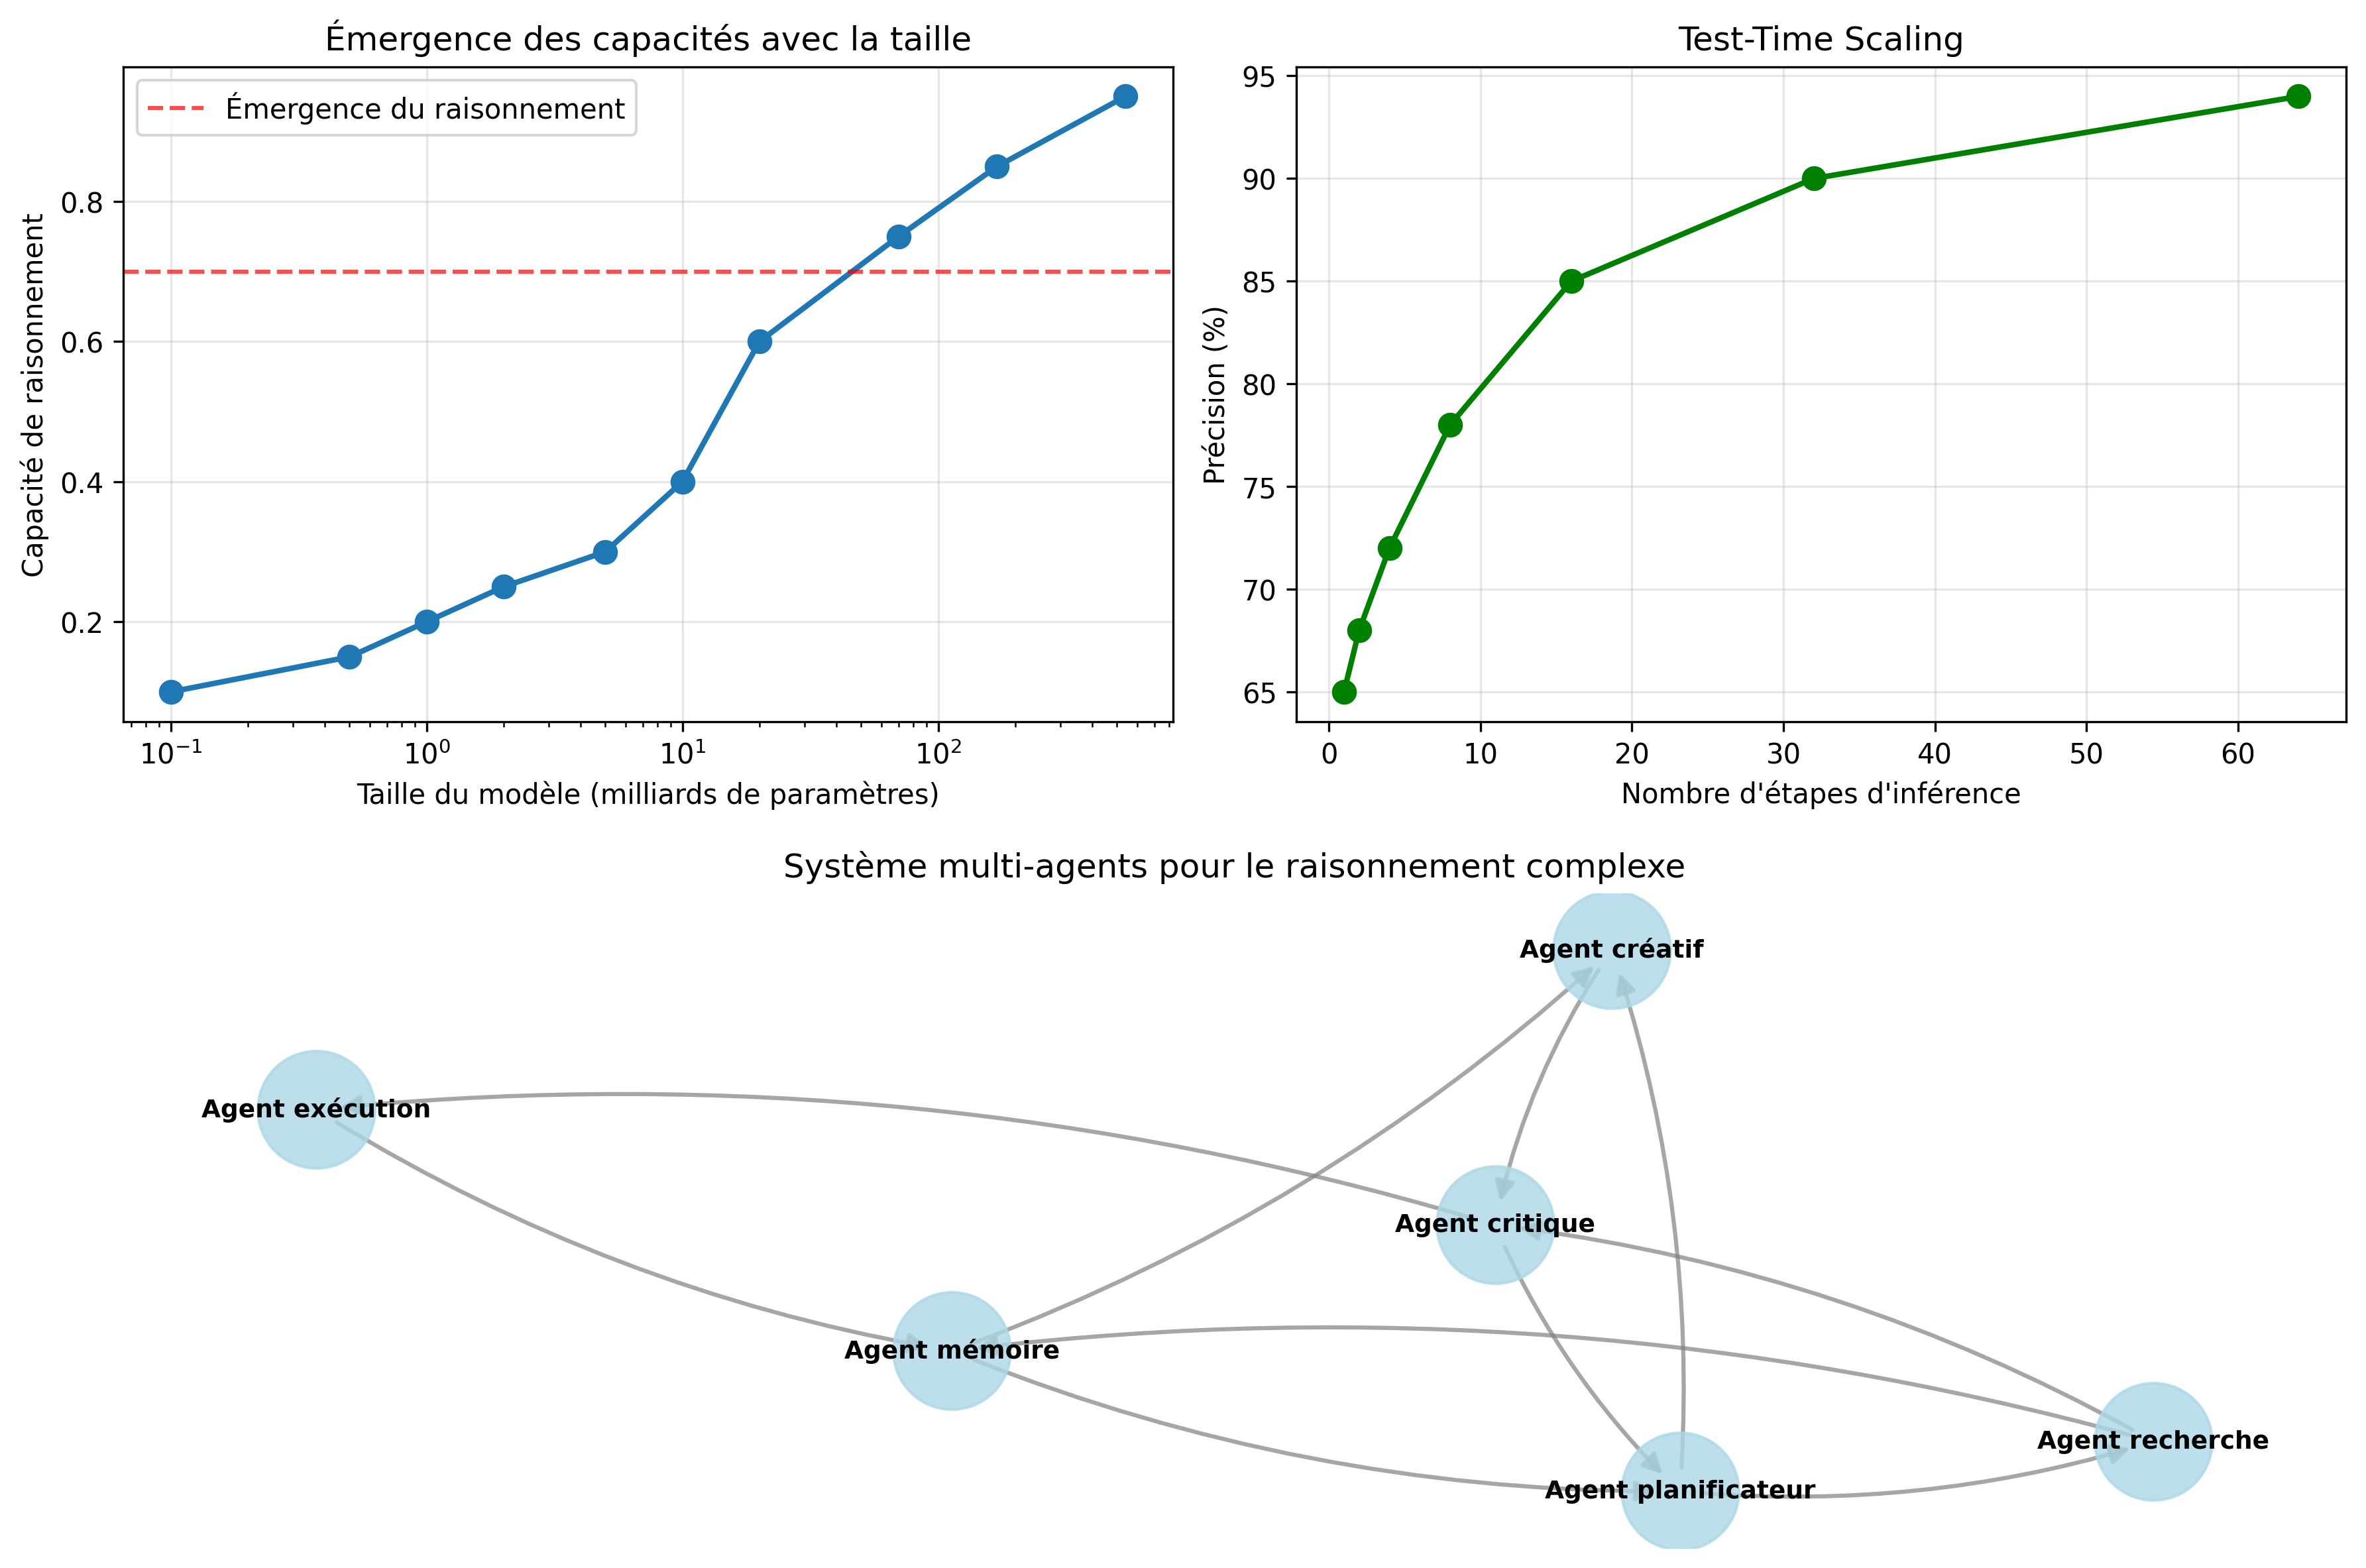
\includegraphics[width=\textwidth]{images/generated/llm_future.png}
            \vspace{0.2cm}
            \begin{center}
                \small{Émergence des capacités et test-time scaling}
            \end{center}
        \end{column}
    \end{columns}
\end{frame}

% Slide: Agent systems and complex interactions
\begin{frame}{Systèmes d'Agents: Intelligence Collective}
    \begin{itemize}
        \item \textbf{Systèmes multi-agents}:
        \begin{itemize}
            \item Plusieurs LLMs spécialisés collaborant sur des tâches complexes
            \item Chaque agent possède un rôle spécifique: planification, critique, recherche, etc.
            \item Communication inter-agents pour résoudre des problèmes multi-étapes
        \end{itemize}
        \vspace{0.3cm}
        \item \textbf{Avantages}:
        \begin{itemize}
            \item \textbf{Auto-correction}: les agents peuvent se critiquer mutuellement 
            \item \textbf{Diversité de perspectives}: différentes approches pour un même problème
            \item \textbf{Spécialisation}: agents optimisés pour certaines tâches spécifiques
            \item \textbf{Réduction des hallucinations}: vérification croisée des informations
        \end{itemize}
        \vspace{0.3cm}
        \item Applications: recherche scientifique, résolution de problèmes complexes, diagnostic médical, création de contenu
    \end{itemize}
\end{frame}

% Slide: Current challenges and future directions
\begin{frame}{Défis Actuels et Directions Futures}
    \begin{columns}
        \begin{column}{0.48\textwidth}
            \textbf{Défis}
            \begin{itemize}
                \item \textbf{Hallucinations}: génération d'informations incorrectes
                \item \textbf{Biais et équité}: reproduction de biais présents dans les données
                \item \textbf{Alignement}: garantir que les modèles agissent selon les valeurs humaines
                \item \textbf{Efficacité énergétique}: réduire l'empreinte environnementale
                \item \textbf{Sécurité}: prévenir les usages malveillants
            \end{itemize}
        \end{column}
        \begin{column}{0.52\textwidth}
            \textbf{Directions de recherche}
            \begin{itemize}
                \item \textbf{Modèles plus petits mais spécialisés}
                \item \textbf{Apprentissage continu} à partir de l'interaction humaine
                \item \textbf{Intégration de connaissances externes} (outils, bases de données)
                \item \textbf{Amélioration de l'interprétabilité} des modèles
                \item \textbf{Multilinguisme} et accessibilité mondiale
                \item \textbf{Multimodalité}: vision, audio, texte combinés
            \end{itemize}
        \end{column}
    \end{columns}
    \vspace{0.3cm}
    \begin{center}
        \textbf{Le futur du NLP se dirige vers des systèmes hybrides intégrant LLMs, bases de connaissances, et outils spécialisés}
    \end{center}
\end{frame}

\end{document} 